\documentclass[preprint]{aastex} 

\usepackage[top=1in, bottom=1in, left=1in, right=1in]{geometry}
\usepackage{amsmath}
\usepackage{graphicx}
\usepackage{mdwlist}
\usepackage{natbib}
\usepackage{natbibspacing}
\setlength{\bibspacing}{0pt}
\setlength{\parskip}{0pt}
\setlength{\parsep}{0pt}
\setlength{\headsep}{0pt}  
\setlength{\topskip}{0pt}
\setlength{\topmargin}{0pt}
\setlength{\topsep}{0pt}
\setlength{\partopsep}{0pt}
\setlength{\footnotesep}{8pt}
\pagestyle{empty}
\citestyle{aa}

%Project Description (8-pages maximum), including the following:
%- A statement of which of the four categories of MSIP is most appropriate
%for this proposal as the first sentence (see section II. Program Description).
%- A scientific justification. For Open Access Capabilities, explain the
%uniqueness and lack of general availability of the capability.
%- A description of the broader impacts, including student training.
%- A description of benefits to the community (observing time, data products, etc.)
%- An outline of the project management plan (where appropriate).
%Note: Results from Prior NSF Support should not be included. Links to URLs may
%not be used.

\begin{document}
\title{Hydrogen Epoch of Reionization Array}
%\title{HERA: Characterizing our Cosmic Dawn} % ARP: this title?

% A statement of which of the four categories of MSIP is most appropriate
%for this proposal as the first sentence (see section II. Program Description).

%This proposal targets the Mid-Scale Science Projects category of the Mid-Scale Innovations Program solicitation. The Hydrogen Epoch of Reionization Arrays (HERA) is a program for using the unique capabilities of the 21cm hyperfine line to trace neutral hydrogen through the cosmic dawn of our Universe.  The HERA roadmap that was submitted to the {\it New Worlds, New Horizons of Astronomy and Astrophysics} 2010 decadal survey, (hereafter NWNH) was given ``top priority in this [Radio, Millimeter, and Sub-millimeter] category of recommended new facilities for mid-scale funding." The HERA roadmap proceeded in three stages: HERA-IB called for \$25M to complete the PAPER and MWA experiments; HERA-II budgeted \$62M for an array with 0.1 km$^2$ of collecting area capable of characterizing the power spectrum of cosmic reionization in detail; HERA-III targeted 1 km$^2$ of collecting area to image reionization structures in detail.

This proposal targets the Mid-Scale Science Projects category of the  Mid-Scale Innovations Program solicitation.

\vspace{0.25in}

\noindent
The major stages in the history of our Universe are written in the phases of hydrogen. The Hydrogen Epoch of Reionization Arrays (HERA) roadmap is a staged program that uses the unique properties of redshifted 21~cm neutral hydrogen emission to study the birth of the first stars and galaxies.  HERA was given the ``top priority in this [Radio, Millimeter, and Sub-millimeter] category of recommended new facilities for mid-scale funding" as part of the {\it New Worlds, New Horizons of Astronomy and Astrophysics} decadal survey, (\citealt{astro2010}; hereafter Astro2010).  

The HERA roadmap envisioned a series of radio interferometers constructed throughout the decade, starting with the PAPER and MWA instruments (Donald C. Backer Precision Array for Probing the Epoch of Reionization; Murchison Widefield Array) aimed at detailed characterization of the foregrounds and first efforts to detect the Epoch of Reionization (EoR) power spectrum, a second-generation instrument to measure the EoR power spectrum in detail and reveal how early structure in the universe formed, and a third-generation instrument late in the decade to image the EoR. 

Using the advances spearheaded by the MWA and PAPER experiments, we are proposing to build the second-generation HERA instrument to extract the exciting science offered by 21~cm observations of the first stars and galaxies. 

In \S \ref{SJsec} we describe the science HERA will enable. Section \ref{LessonsSec} then reviews the breakthroughs in our understanding the EoR foregrounds from PAPER and MWA, and the techical heritage which allows HERA to perform the science envisioned in the decadal survey at significantly reduced cost. The full HERA instrument and timeline is described in \S \ref{PDsec}, followed by the impacts on the US scientific and national community in \S \ref{BIsec}.


\vspace{-0.25in}
\section{Scientific Justification}
\label{SJsec}

The period beginning with the birth of the first luminous objects in the
universe, and culminating with the ionization of the intergalactic medium (IGM)
$\sim$500 Myrs later, is one of the last unexplored phases of cosmic evolution.
Exploring this epoch of reionization was highlighted as one of the three
``priority science objectives chosen by the [NWNH] survey committee for the
decade 2012-2021" \citep{astro2010}. Observations of Gunn-Peterson absorption
by the IGM toward the most distant quasars \citep{fan_et_al2006}, kinetic
Sunyaev-Zel'dovich features in the CMB \citep{zahn_et_al2012}, and CMB
anisotropy and polarization \citep{page_et_al2007,planck_et_al2013} indicate
that reionization was a complex process, starting perhaps as early as 
$z\approx14$, with the last vestiges of the the neutral IGM being etched away by
$z\approx6$.  Unfortunately, these ground-breaking results are limited in
diagnostic capabilities: the Gunn-Peterson effect saturates for even low
neutral fractions, and the CMB only provides an integral measure of the
Thompson optical depth back to recombination.

Redshifted emission from the 21cm hyperfine transition of neutral hydrogen has
gained considerable attention as a unique (albeit weak) tracer of the
primordial IGM.  The direct observation of the neutral IGM via this signal
would be an achievement comparable with the discovery of the CMB.  As
emphasized in NWNH \citep{astro2010}: ``The panel concluded that to explore the
discovery area of the epoch of reionization, it is most important to develop
new capabilities to observe redshifted 21-cm HI emission, building on the
legacy of current projects and increasing sensitivity and spatial resolution to
characterize the topology of the gas at reionization."

\begin{figure}[!ht]\centering
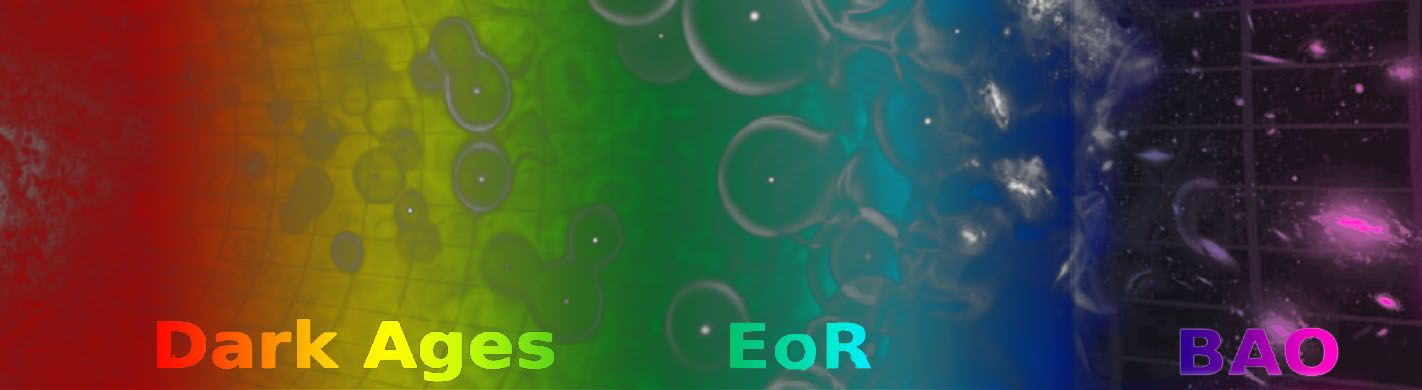
\includegraphics[width=6in]{plots/21cm_cosmo.jpg}
\caption{\small
The 21cm hyperfine line of neutral hydrogen represents the next frontier in
precision cosmology. Following recombination (left edge), the spin temperature
of 21cm emission is sensitive to the density and temperature of the
intergalactic medium (IGM) through the Dark Ages, evolves with the heating and
ionization of the IGM during the Epoch of Reionization (EoR), and
traces the distribution of galaxies as the universe expands,
leading up the the present day (right edge).  Color indicates
redshift, which stretches the 21cm line to frequencies ranging from 50 MHz
(red) to 1.4 GHz (violet).
}\label{fig:21cm_cosmo}
\end{figure}

The challenges associated with 21cm cosmology experiments are daunting.  Such
experiments require unprecedented levels of sensitivity, instrumental
calibration, and foreground characterization.  The spectral response of these
instruments is of paramount importance; it is used both for constructing the
line-of-sight direction of 3D space, and also for differentiating
smooth-spectrum foreground emission from spatial fluctuations in the
cosmological signal. The brightness temperatures of foregrounds, in the form of
galactic synchrotron emission, continuum point-sources, and polarized
galactic/extra-galactic emission, exceed the fluctuations of the 21cm signal by
more than 5 orders of magnitude
\citep{santos_et_al2005,pritchard_loeb2012,pober_et_al2013b}.

As is being discovered, these foregrounds are proving very difficult to attack
head-on.  To achieve the necessary sensitivity, experiments are driven toward
using interferometers, but the frequency dependence of the angular wavemode
sampled by an interferometer causes smooth-spectrum foregrounds to appear
unsmooth, degrading the separation that can be achieved between foregrounds and
$k$-modes of the 21cm power spectrum $\Delta^2_{21}(k)$.  
%XXX maybe remove jargon here and describe consensus of community around “the wedge”.
Experimental approaches adopted by LOFAR and the MWA aim to achieve sufficient
accuracy in foreground characterization and instrument calibration to model and
remove such chromatic effects.  However, this is proving to be an extremely
challenging and costly task, and it remains uncertain whether this approach is
practically viable given realistic limitations on calibration accuracy.

\begin{figure}[!ht]\centering
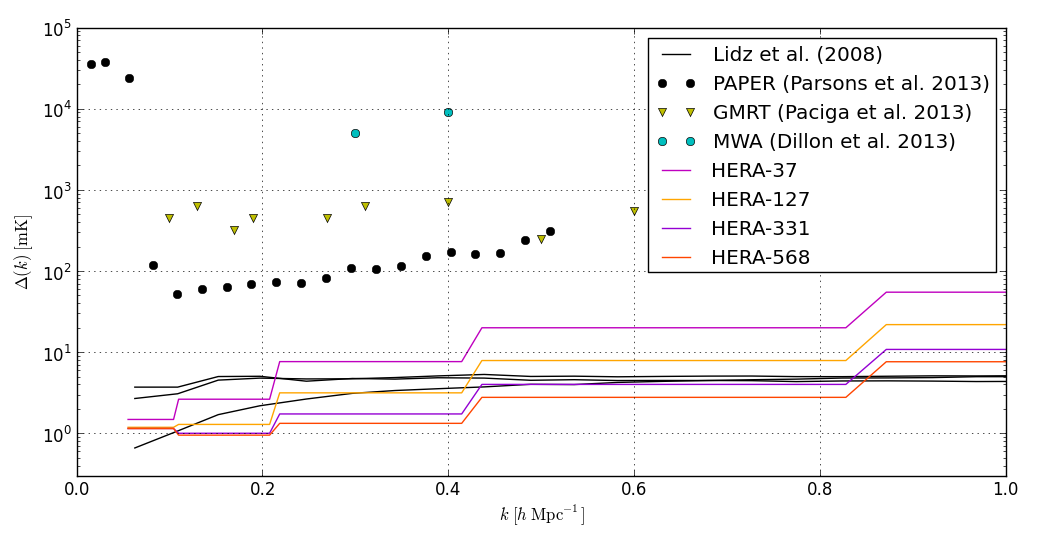
\includegraphics[height=3.0in]{plots/eor_pspec.png}
\caption{\small
Current best upper limits on the power spectrum of 21cm emission from
reionzation at $z=7.7$, made with a 32-antenna deployment of the PAPER
experiment \citep{parsons_et_al2013}. Black indicates the final measurements
with 2$\sigma$ confidence intervals. The yellow triangles indicate the previous
best 2$\sigma$ upper limits at $z=8.6$ \citep{paciga_et_al2013}. Magenta
illustrates a fiducial 50\% ionization model \citep{lidz_et_al2008}. The 8
orders of magnitude (in mK$^2$) of foreground suppression outside of the dashed
lines (left panel) are a testament to the crucial role that instrument design
plays in mitigating foreground systematics.
}\label{fig:eor_pspec}
\end{figure}

PAPER has made significant progress following a different approach.  Based on a
``delay-spectrum'' understanding of the mechanism for how instrumental
responses modulate foregrounds on spectral scales of cosmological interest
\citep{parsons_et_al2012b}, PAPER has optimized its instrument to focus on
regions in Fourier space that have weak coupling to foregrounds. XXX describe
optimization to foreshadow changes in HERA.  These regions are determined both
by chromatic instrumental responses and by the inherent frequency evolution of
the foregrounds.  As shown in Figure \ref{fig:eor_pspec}, observations based on
this new approach are demonstrating that the extremely stringent level of
foreground removal needed to access the 21cm signal is largely in hand, with
upper limits that are beginning to rule out cold reionization scenarios. 



\vspace{-0.25in}
\section{Lessons learned from PAPER and MWA}
\label{LessonsSec}

Talk about the window and current limits.

\begin{figure}\centering
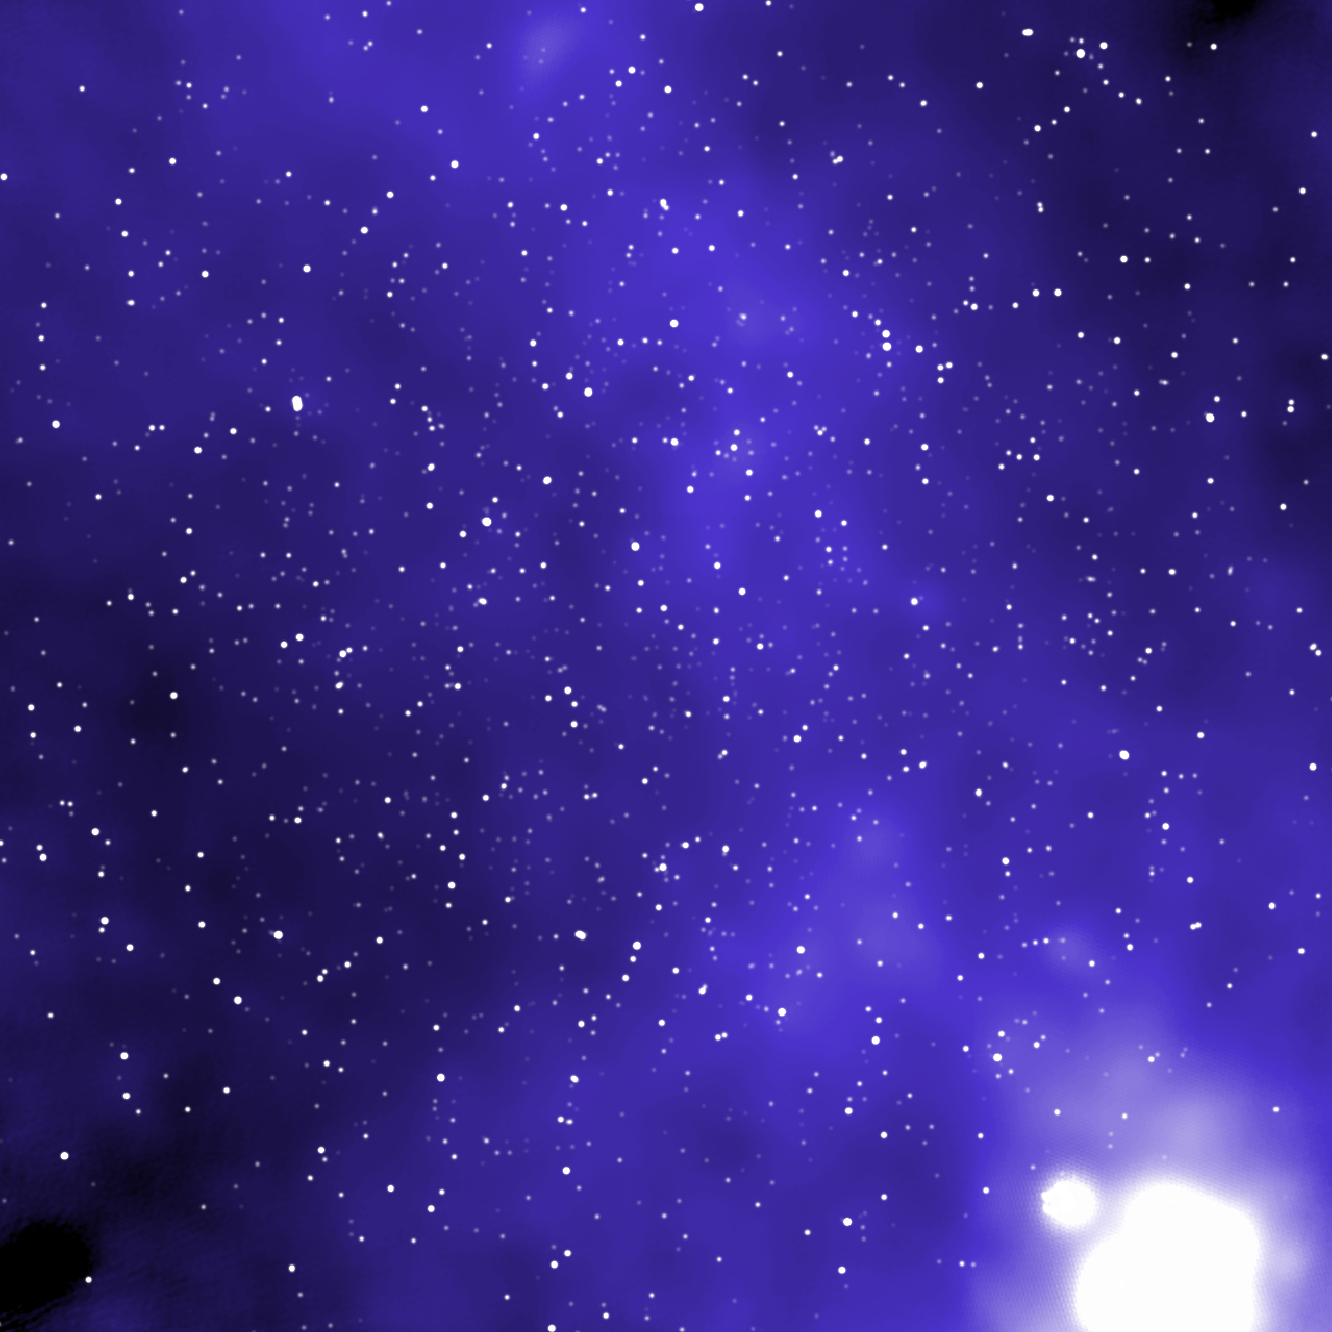
\includegraphics[width=6.5in]{plots/MWApretty.png}
\caption{\small
High dynamic range imaging of foregrounds with the MWA towards galactic center utilizing the Fast Holographic Deconvolution software package developed at the University of Washington. Vela and Puppis SNRs are in the lower right, and the image is approximately $30^{\circ}$ in diameter. Analysis includes direction dependent beam and polarization effects, and routinely achieves $<0.5\%$ polarization leakage across the field. Subtracting precision maps of smooth spectrum and polarized foregrounds will enable HERA to enlarge the EoR window.
}\label{fig:prettyPicture}
\end{figure}

\begin{figure}\centering
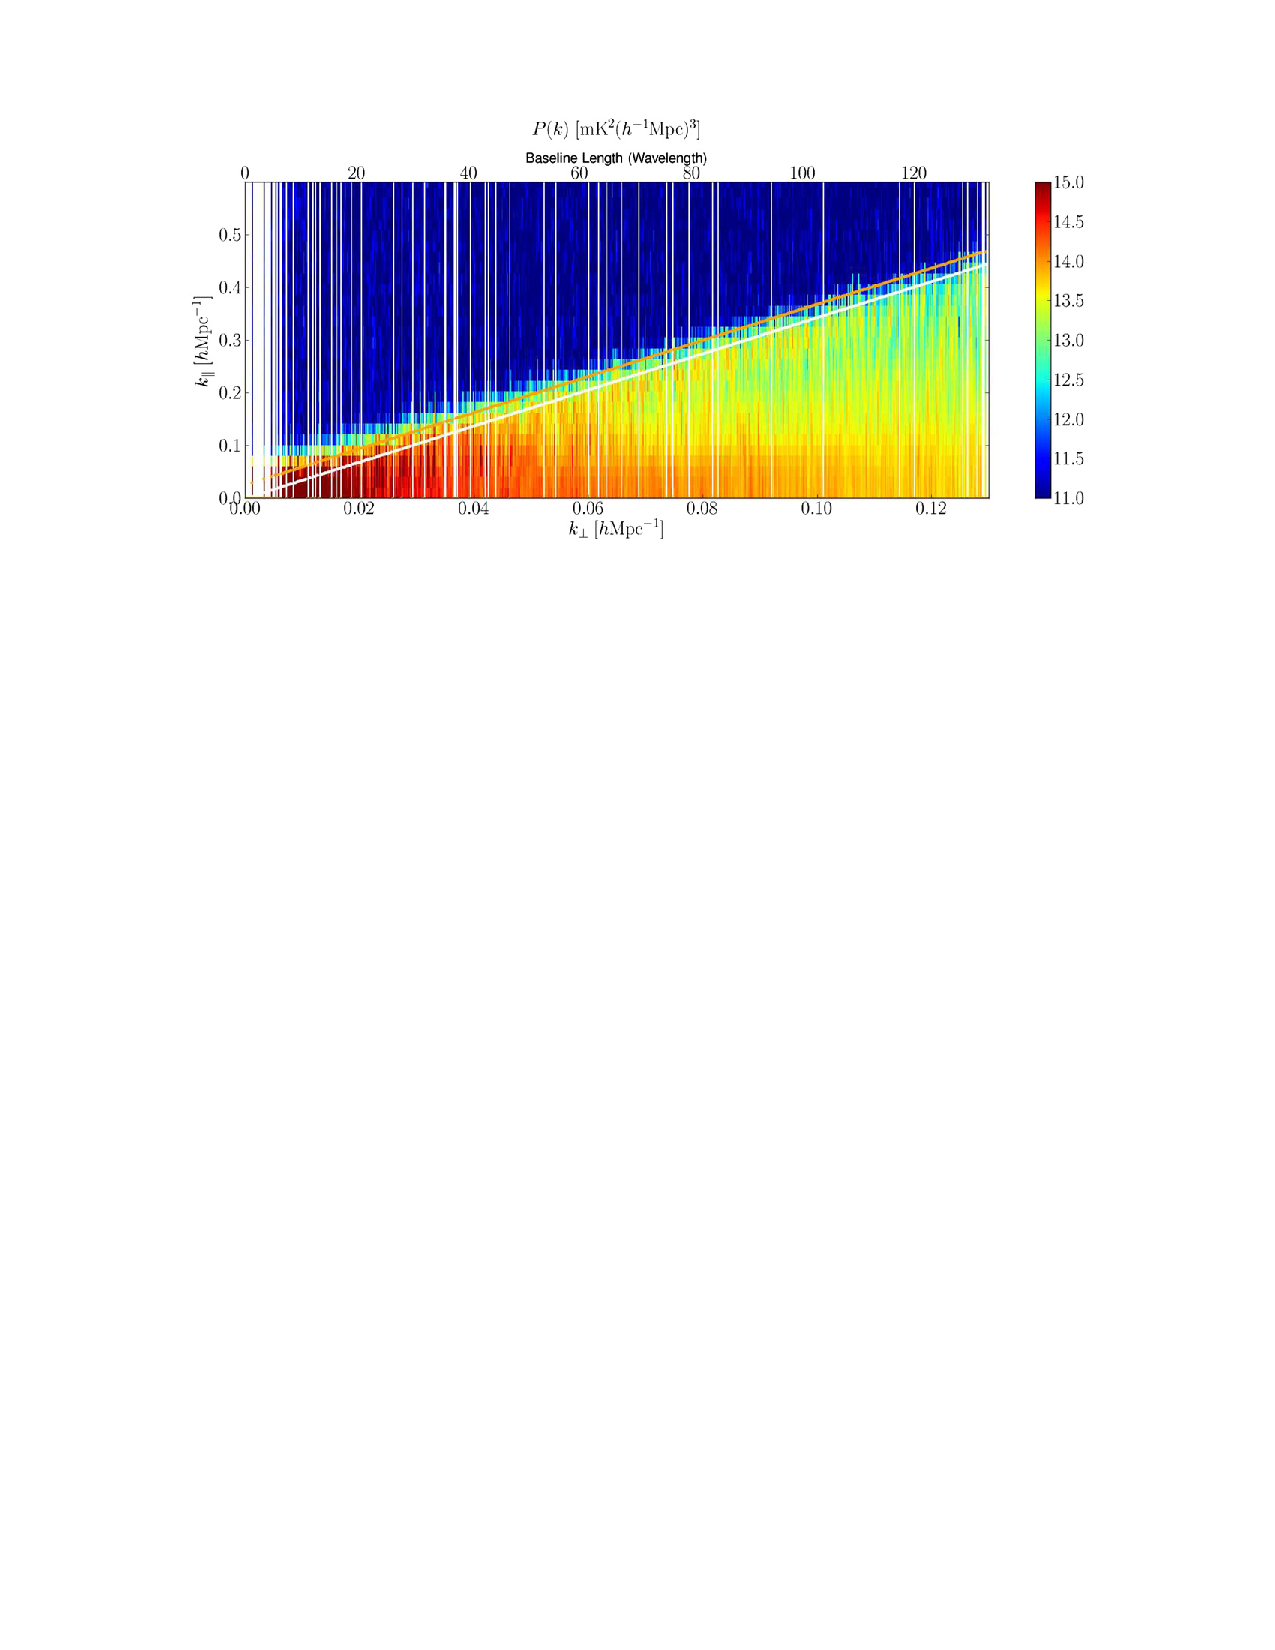
\includegraphics{plots/Pober_wedge.pdf}
\caption{\small
The EoR window as measured by PAPER.  Blue represents a region containing EoR signal but no foreground contamination.
}\label{fig:EoRwindow}
\end{figure}




\vspace{-0.25in}
\section{Project Description}
\label{PDsec}

\begin{figure}[!ht]\centering
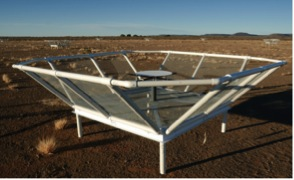
\includegraphics[height=1.75in]{plots/paper_element.jpg}
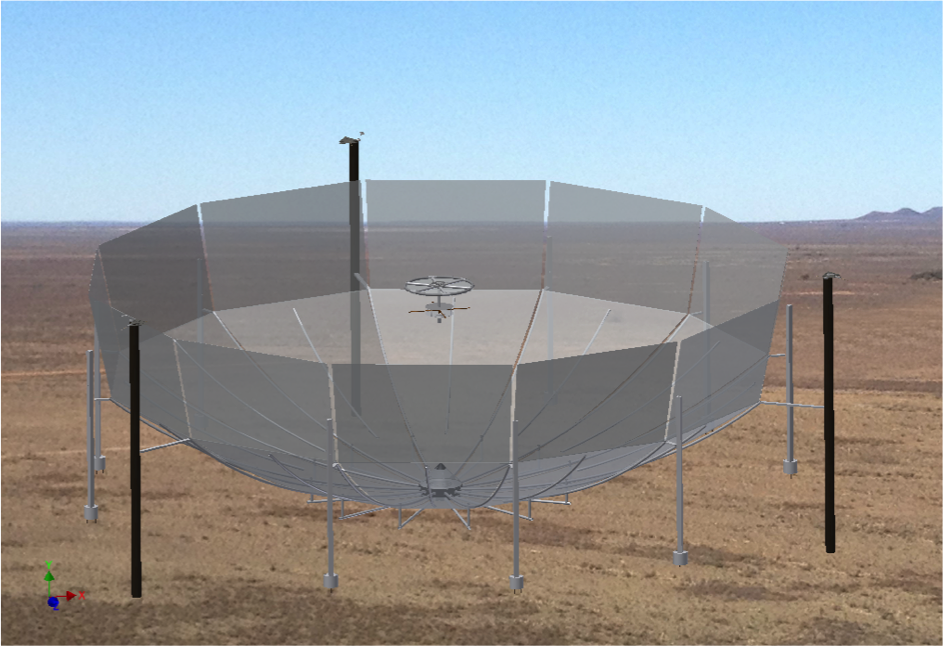
\includegraphics[height=1.75in]{plots/hera_dish.png}
\caption{\small
The PAPER element (left) provides a clean instrumental response as a function
of frequency \citep{parsons_et_al2010,parsons_et_al2012b}, which is crucial to
the foreground isolation shown in Figure \ref{fig:eor_pspec}.  A 14~m dish
designed around the same feed (right) dramatically improves sensitivity while
constraining the path length and amplitude of
reflections to ensure that foreground isolation is not substantially degraded.  
}\label{fig:hera_dish}
\end{figure}

This proposal outlines a staged build out to a 568-antenna array in South Africa that incorporates the lessons learned from the first generation EoR observatories. It features a 14~m zenith pointing dish optimized for spectral smoothness, a dense hexagonal core to enable redundant baseline calibration and delay-spectrum analysis, and a distribution of outrigger antennas to provide complete uv coverage to $\sim$700~m for foreground imaging and mitigation. HERA draws on the technical heritage of the MWA, PAPER, and EDGES. Specific examples include the spectrally smooth feed and antenna based on PAPER, receiver node and field digitization at baseband from the MWA, absolute radiometric calibraion from EDGES, the delay-spectrum analysis from PAPER, and the precision imaging and foreground removal software from the MWA.

The HERA antenna shown in Figure \ref{fig:hera_dish} is an illustrative example of how the HERA design has been optimized based on our current understanding. The key antenna figure of merit is the spectral smoothness and stability of the response because it determines the precision to which astrophysical foreground emission can be separated from the cosmological 21~cm emission. HERA uses the PAPER dipole feed---modified slightly for wider bandwidth---suspended over a 14~m parabolic dish. The short ($\sim$5m) focal height of the dishes is central to limiting the path length of reflections whose time-delay gives rise to chromatic antenna sensitivity. The zenith pointing enhances the stability of the antenna response (PAPER), short cables to in-field digitizers limit the length of cable reflections (MWA), and absolute calibration (EDGES) are all designed to provide an extremely stable and smooth spectral response. Similarly the antenna layout uses the dense core, outriggers, and symmetric configuration of the MWA, combined with redundant baselines within the core (PAPER). Together these advances enable HERA to have the science reach envisioned in the decadal survey while fitting within the MSIP funding envelope.

%This HERA proposal targets a 568-element array that incorporates these proven
%foreground avoidance techniques while addressing the sensitivity limitations of
%current experiments.  With a better understanding of how antenna size and
%separation affect the interaction of sensitivity and foreground isolation, it
%has become clear that larger, close-packed antenna elements can yield up to 30
%times the sensitivity of current elements without substantially degrading
%foreground isolation.  Where PAPER’s elements lack collecting area and are
%smaller than strictly required for foreground isolation, and the majority of
%MWA and LOFAR elements are spaced too widely to avoid foregrounds, HERA employs
%an extremely compact array of large --- but not {\it too} large --- antenna
%elements, building on PAPER's design.  As illustrated in Figure
%\ref{fig:hera_dish}, these elements consist of PAPER-style dipole feeds
%suspended over 14m parabolic dishes.  The short ($\sim$5m) focal height of these
%dishes is central to limiting the path length of reflections whose time-delay
%gives rise to chromatic instrumental systematics. 

%The size of the new HERA dish optimizes cost for a fixed sensitivity and level
%of foreground isolation.  The associated reduction in the number of antenna
%elements, combined with the fact that these dishes have no moving parts, are
%built from inexpensive materials, and follow a simple construction that can be
%delegated to local contractors, makes the cost of building HERA's Phase-II
%experiment several times cheaper than was anticipated in the HERA roadmap
%endorsed by Astro2010.  
%XXX talk a bit more about build-ability.

HERA follows a staged build-out plan.  In
each deployment stage improvements are incorporated into the system and new
science capabilities are unlocked.  This approach has the advantage of
providing early access to science and reducing the project risk by testing systems
early and changing them incrementally.  As shown in Figure \ref{fig:eor_pspec}, each
stage of HERA brings an associated improvement in sensitivity that allows key
aspects of 21~cm reionization science to be addressed.  The timeline of HERA
development, along with the associated science products, is outlined below. 


\noindent{\bf Year 1--Infrastructure and First 37 Antennas (FY 2015)}.  
\begin{itemize}\setlength{\parskip}{0pt}
\vspace{-7pt}
  \item Infrastructure installation. Using the new `K3' site approximately 10~km from the current PAPER site at the Karoo Radio Observatory in South Africa. Includes ground leveling, power and basic network connectivity.
  \item Move existing PAPER-128 antennas, correlator, and EMC container to K3 site.
  \item Install first 37 HERA antennas and instrument with existing PAPER feeds and electronics. 
  \item Begin development of wider bandwidth HERA baluns, receivers, feeds, and nodes using the PAPER and MWA techical heritage \citep{} and the development of in-situ antenna calibration system based on EDGES \citep{}. Continue development of delay-spectrum \citep{} and Fast Holographic Deconvolution software (FHD; \citealt{}).
\end{itemize}


\noindent{\bf Year 2--Hardware Commissioning and Deep Foreground Survey (FY 2016)}.  
\begin{itemize}\setlength{\parskip}{0pt}
\vspace{-7pt}
  \item Commissioning observations using a hybrid array of 37 HERA antennas in a close-packed hexagon surrounded by 91 PAPER antennas in an imaging configuration.
  \item Perform a deep polarized foreground survey using unique hybrid antenna capability of FHD. Will directly determine on-sky beam response of HERA antennas and enable future subtraction of sources in HERA sidelobes.
  \item Finalize site infrastructure (high-bandwidth optical network, surveying, trenching).
  \item On-antenna commissioning of new feeds, receivers, nodes, and antenna calibrations systems in Green Bank and South Africa.
  \item Build out to 127 HERA antennas starts.
\end{itemize}


\noindent{\bf Year 3--HERA 127 and Detecting the Rise and Fall of Reionization (FY 2017)}.
\begin{itemize}\setlength{\parskip}{0pt}
\vspace{-7pt}
  \item Construction of HERA-127 completes, and science observations begin in Oct. 2016, again using the PAPER correlator.
  \item Analysis begins on a dataset capable of constraining the timing and duration of reionization. Analysis focuses on current techniques based on PAPER individual baseline analysis, with exploration of subtracting bright and polarized foreground sources.
  \item Deployment of HERA~331 begins. Node electronics are installed for all 331 elements, and a new, 331-element GPU-based correlator is installed in the Karoo Array Processing Building (KAPB).
  \item Science papers from HERA-37 are published.
  \item  Additional data storage infrastructure is installed in the
KAPB.  The UPenn data analysis cluster is upgraded. 
\end{itemize}

\noindent{\bf Year 4--HERA 331 and Measuring the Evolution of the First Galaxies (FY 2018)}.
\begin{itemize}
\setlength{\parskip}{0pt}
\vspace{-7pt}
  \item Construction of HERA~331 completes, and science observations begin in Oct. 2017.
  \item Science observations with HERA~331 complete in Apr. 2018, and analysis begins on a dataset capable of
characterizing the redshift evolution the power spectrum shape---measuring the development of the first galaxies.
  \item Continued analysis and software development with an emphasis on opening the EoR window (removing contamination at low $k_{\parallel}$). 
  \item  HERA~127 results are published.
  \item Build out to 568 antennas begins, including outrigger antennas to fascilitate imaging and better foreground removal.
  \item Pipelines for EoR processing of HERA~568 complete.
\end{itemize}

\noindent{\bf Year 5--HERA 568, Imaging Reionization and Constraining the Development of Structure at $z>11$  (FY 2019)}.
\begin{itemize}
\setlength{\parskip}{0pt}
\vspace{-7pt}
  \item Construction of HERA~568 completes, and science observations begin in Oct. 2018.
  \item Analysis push to enable imaging of the largest structures and extracting the full sensitivity of the instrument (including partially coherent baselines). 
\end{itemize}




\subsection{The Transformative Science enabled by HERA}

% XXX Talk about specifically what science is being added in each stage of HERA
% XXX Bowman plot of constraints on ionization fraction versus redshift
% XXX new capabilities that are added in each stage
% XXX new low-frequency exploration, dark-ages plot from Aaron Ewall-Wice

\section{Broader Impacts and Benefit to the Community}
\label{BIsec}



\subsection{Developing Young Instrumentalists (shorten)}
Aspiring instrumentalists in radio astronomy face a challenging path, in part because
the fundamental nature of radio astronomy instrumentation is changing.
Because the capabilities of radio telescopes are directly tied to the Moore's Law
growth in the capabilities of digital electronics,
new science opportunities are constantly being opened up, while existing
facilities rapidly fall into obsolescence.
Furthermore,
the breakneck pace of technological development places a premium on rapid development.
The faster an instrument incorporating new technology can be deployed,
the earlier that new science goals can be reached.

All of this combines to mean that aspiring radio astronomy instrumentalists must acquire a very broad
set of skills in a short amount of time.  A sampling of the skills required includes the practical
application of antenna design, optics,
3D modeling, machining, circuit design, soldering, DSP algorithms, FPGA/GPU programming, network management,
computing systems, kernel optimization, interferometry, synthesis imaging, astrometry, statistical methods, linear
algebra, high-performance
computing, laboratory methods, and many, many others.  While some of these skills are taught
in undergraduate and graduate
curricula, many are not, and exposure varies tremendously between majors.  In particular,
many students who arrive at graduate school in astronomy and physics
lack preparation in
practical engineering, programming, and laboratory skills.  Students with talent in physics, math, and astronomy,
but with a practical bent are often siphoned off in other directions.

One aspect of the broader impact of this proposal addresses the loss of talented
scientists with practical skills from applications in astronomy
instrumentation, and to address the gap between the preparation afforded by an
undergraduate education and the breadth of skills required to succeed as an
aspiring (radio) instrumentalist in graduate school.  This will be done by
funding a one-year junior specialist position in the RAL, offered annually over the course of this grant, to a
person to who
will gain practical experience working alongside professional RAL engineers and scientists
on all aspects of the HERA instrumentation development at UC Berkeley, with the goal of
acquiring the practical skills required for
pursuing research in instrumentation in a graduate program.

\subsection{Developing African Scientists}

(Carilli)

\subsection{Benefits to the Community: Data Products (needs work!)}

(Carilli) benefit/synergy with JWST, WFIRST, CMB pol stuff, etc.
Data products disseminated at MIT.  Products include:
integrated data products, made available after 2 years;
high-speed continuum images, generated as part of operational data analysis by MIT;
wide-field sky maps (made with 91 PAPER antennas in first 2 years),
database of metadata  for asscoiated with data products,
access to calibrated, compressed visibilities upon request.
deep (foreground subtracted) image products for use with other surveys \& instruments

\section{Project Management Plan}

This project strikes a balance between the light-weight
management structure of HERA-I activities and the more formal structure
required for larger-scale projects.  Building on PAPER's excellent track record
and the resources of UC Berkeley's Radio Astronomy Laboratory (RAL),
this proposal consolidates responsibility and management of the core HERA
fabrication and construction activities at RAL. Parsons serves as
Project Director/Scientist; DeBoer serves as Project Manager/Engineer.
Executive
(Aguirre, Bradley, Hewitt, Morales, Werthimer)
and Scientific (Aguirre, Bowman, Carilli, Furlanetto, Hewitt, Morales, Tegmark) Advisory Boards advise Parsons.
A Site Manager will supervise and manage
construction activities executed by local contractors at the South African
site, and reports to DeBoer.  A SKA-SA Liaison (supported by SKA-SA)
interacts with DeBoer, the Site Manager and the SKA-SA board to
coordinate HERA, Meerkat and SKA site activities.

An external advisory board evaluates the baseline design
based on existing components in a Preliminary Design Review in Year 1.
A Critical Design Review in Year 2 evaluates the
production design, incorporating improvements to the analog system
and feeds (Bradley), the node and correlator (Werthimer), and the data storage
system (Aguirre), and analysis software (Morales).
Fabrication of sub-systems (electronics, antenna sub-assemblies and antenna assembly)
are contracted to industry, both in the US and South Africa.   Construction on site proceeds
with 2-3 teams of local contractors and laborers, managed by the UCB-appointed site manager.  Observing proceeds autonomously without local observers; SKA-SA
provides occasional site support as necessary.

Project risk and contingency are handled primarily by de-scoping along the axes of scale, time and new capability.  Baseline designs using
existing hardware establish a low-risk path to basic functionality yielding new science.  Improved functionality
results from successful development activities or is otherwise de-scoped.
Cost excesses and schedule slips are absorbed by reducing
build-out, with associated de-scoping of science capabilities.

%\begin{table}
%\label{tab:params}
%\begin{tabular}{|l|rl|l|}
%\hline
%Parameter & Value & Units & Description \\
%\hline
%$N$  &  576  & & Number of Antennas \\
%$d$ & 14 & m & Antenna Diameter \\
%$f/d$ & 0.32 &  & Focal Length (fractional) \\
%$\Omega_{\rm P}$ & 0.026 & sr & Field of View (power) \\
%$\Omega_{\rm PP}$ & 0.013 & sr & Field of View (power$^2$) \\
%$\Omega_{\rm eff}$ & 0.052 & sr & Field of View (sensitivity) \\
%$B_{\rm samp}$ & 0--250 & MHz & Sampled Frequency Range \\
%$B_{\rm corr}$ & 100 & MHz & Correlated Bandwidth \\
%Config.    & 24 $\times$ 24 & & Square Grid Antenna Configuration\\
%$f/f_0$ & $1.5\cdot10^5$ & & Redundancy Metric (Parsons et al. 2012a) \\
%$A$ & 0.09 & km$^2$ & Total Collecting Area \\
%$\theta$ & 15 & arcmin & Angular Resolution (150 MHz) \\
%$b_{\rm max}$ & 500 & m & Maximum Baseline \\
%$T_{\rm sys}$ & 500 & K & System Temperature \\
%$t_{\rm obs}$ & 120 & days & Observing Time \\
%$t_{\rm day}$ & 6 & hrs & Observing Time Per Day\\
%$\Delta_{\rm N}^2$ & 1.6 & mK$^2$ & Expected Noise Level ($k=0.2 h\ {\rm Mpc}^{-1}$) \\
%SNR$_{21}$ & 11.7$\sigma$ &  & Expected Detection Significance (Lidz et al. 2008, $x_i=0.5$, 150 MHz) \\
%\hline
%\end{tabular}
%\end{table}

\clearpage
\setcounter{page}{1}
\thispagestyle{empty}
%\bibliographystyle{apj}
%\bibliographystyle{hapj}
\bibliographystyle{jponew}
\bibliography{biblio}


\end{document}